\documentclass[onecolumn]{article}
%\usepackage{url}
%\usepackage{algorithmic}
\usepackage{geometry}
 \geometry{
 a4paper,
 total={170mm,257mm},
 left=20mm,
 top=20mm,
 }
\usepackage{wrapfig}
\usepackage{datetime}
\usepackage[margin=2em, font=small,labelfont=it]{caption}
\usepackage{graphicx}
\usepackage{mathpazo} % use palatino
\usepackage[scaled]{helvet} % helvetica
\usepackage{microtype}
\usepackage{amsmath}
\usepackage{subfigure}


% Letterspacing macros
\newcommand{\spacecaps}[1]{\textls[200]{\MakeUppercase{#1}}}
\newcommand{\spacesc}[1]{\textls[50]{\textsc{\MakeLowercase{#1}}}}

\title{\spacecaps{\textbf{CENG 3521: Data Mining Final Project}\vspace{0.5cm}
        \large Socioeconomic Status of Countries}\\ \normalsize \spacesc{} }

\author{Çilem Emre - 170709011\\Dilan Bozkurt - 170709020}
%\date{\today\\\currenttime}
\date{}

\begin{document}
\maketitle

\section{Introduction}

In this project, we aim to find out the development level of the all countries by measuring the factors that are determining the socioeconomic level of countries via using clustering strategies. The main purpose of the project is to find the top 10 countries that are in the worst conditions through some factors such as child mortality rates, gross domestic product per person, health, exports, imports and inflation also to find out which factors are contributing in what degree to determine the whether a country is developed or not. With the outcome of this project, we can establish the countries which need the most help from international powers such as United Nations.

\section{Preprocessing}

\begin{center}
    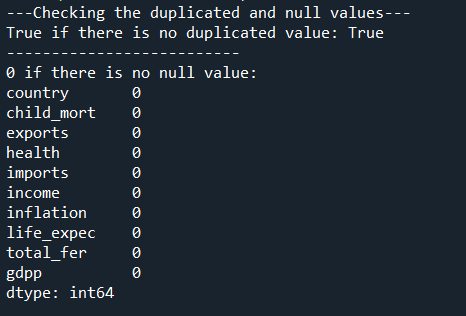
\includegraphics[width=0.50\textwidth]{1.png}
    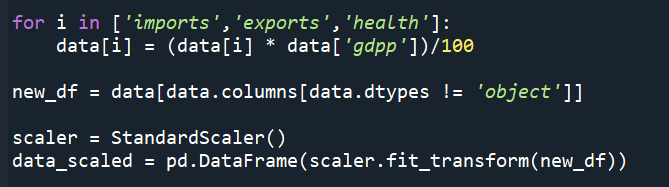
\includegraphics[width=0.50\textwidth]{scaler.PNG}
\end{center}

Data preprocessing is a data mining technique that involves transforming raw data into an understandable format. Real-world data is often incomplete, inconsistent, lacking in certain behaviors or trends, and is likely to contain many errors. Data preprocessing is a proven method of resolving such issues. Data preprocessing prepares raw data for further processing.
After doing data preprocessing, we saw that there are no duplicate and null values in the data as shown. Therefore, we do not need any data cleaning process on the data. \\Also, the export, health, import columns in the data are percentage. To find out their actual value, we multiplied by the "gdpp" column and divided by 100.Additionally, we applied standard scaler to increase the similarity in the data. Most of distance based models e.g. k-means and hierarchical clustering need standard scaling so that large-scaled features don't dominate the variation.
For example, once a feature with large values like income is scaled, we increase the accuracy score.
\normalsize
\section{According to factors, plot the 10 countries that has the worst conditions}

\begin{center}
    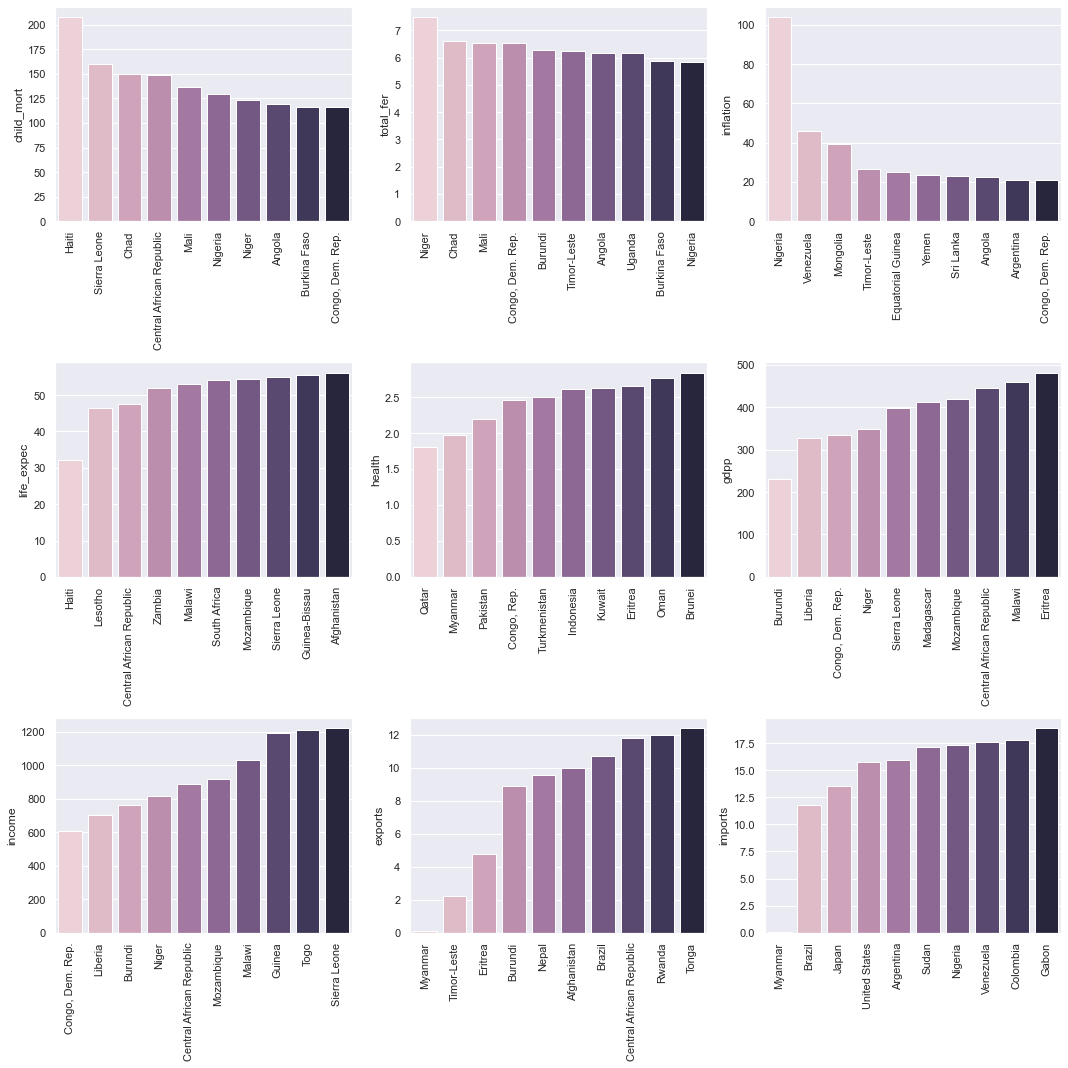
\includegraphics[height=0.25\textheight]{firsfig.png}
\end{center}

The figure at the right side contains the top 10 countries that are doing poorly in the all the factors. The correlation between this figure and the results of the project can help us the detect the which factors are the ones that has most effective.

\normalsize
\section{Clustering}

Clustering methods are used to find similarity and relationship patterns among data samples. After that, they cluster those samples into groups having similarity based on features. In this project, we will try k-means clustering and hierarchical clustering and compare the similarity of the results. 

\subsection{K-Means Clustering}

K-means is a simple iterative clustering algorithm. Starting with randomly chosen K centers, the algorithm proceeds to update the centers and their clusters to equilibrium while minimizing the total within cluster variance. It is primarily used in scenarios with real-valued features because it relies on the Euclidean distance to discover cluster centers.

\subsubsection{Finding the optimum number of clusters with k-means clustering}

We used elbow curve and silhouette score methods to find the optimum cluster number in K-means clustering.

\subsubsection{Elbow Curve}

\begin{center}
    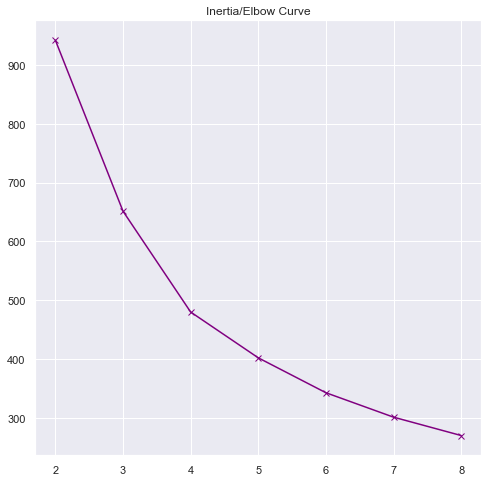
\includegraphics[width=0.45\textwidth]{elbowcurve.png}
\end{center}

\begin{center}
    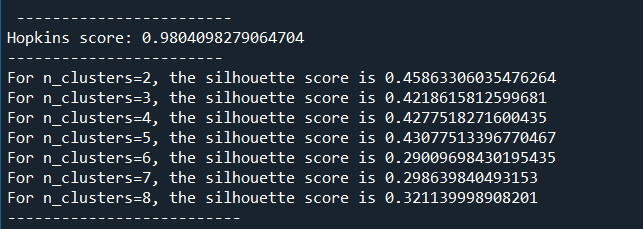
\includegraphics[width=0.50\textwidth]{sil.png}
\end{center}
What is the good number of clusters can be determined with a way called Elbow method. It is based on the sum of squared distance (SSD) between data points and their assigned clusters' centers. The point where the SSD starts to straighten and makes an elbow is usually is the chosen spot. We get this result at 4.
Silhouette analysis is used to looking at the distance between clusters. It get a measure how close each point in one cluster is to points in the neighboring cluster then give a range between -1 to 1.
When we look at the scores, we can see the 2 has the highest one. But we won't use 2 because two clusters are simply not enough for segregating the countries. The results of 3, 4, 5 are similar, at the next step, we will study them and choose the best fitted number. In addition, the Hopkins score determines whether the data is suited for clustering or not, usually 0.70 is good. We get 0.98 so the data is well suited for clustering.

\subsubsection{Plotting the heatmap to see the correlations between variables}

\begin{wrapfigure}{r}{0.50\textwidth} 
    \vspace{\dimexpr0.05\baselineskip-\topskip}%
    \centering
    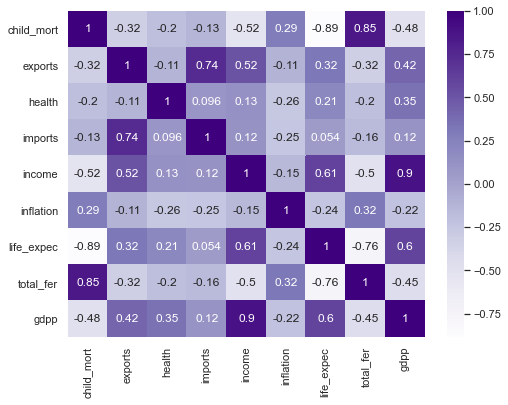
\includegraphics[width=0.50\textwidth]{heatmap.png}
\end{wrapfigure}

Income has positive correlation (0.61) with life expectancy and negative correlation (-0.52) which child mortality. This signifies that countries with higher income values can spend more in healthcare which reduced the child mortality and increases average life expectancy.
GDP and Income has high positive correlation (0.9). This indicates countries where people have high income has high GDP and they tend to prosper more. This is what is expected.
Total Fertility and Child Mortality has high correlation. It may be due to the fact that if child mortality is higher, people tend to opt for more children.
The highest negative correlation is between life expectancy and child mortality.
\normalsize
\subsubsection{Child mortality - Income graph with different clusters}
\begin{center}
    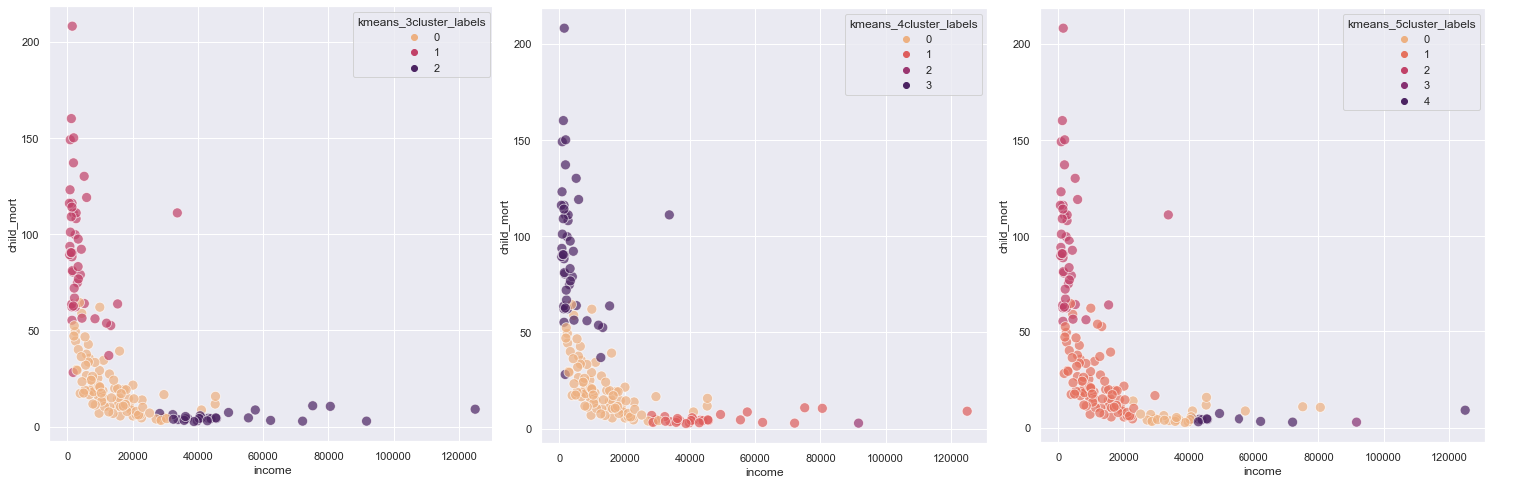
\includegraphics[scale=0.50]{123.png}
\end{center}
\large
In this part, we use the two factors child mortality and income which has very high negative correlation between them. We applied k-means with  3, 4 and 5 clusters and visualized it with seaborn library. At the elbow score figure above we saw that 3 cluster got a higher score than 4 but the difference between them is just one country: Luxembourg which is unusually rich and prosperous. We think Luxembourg should have its own cluster because it has such extreme values. After 2, 5 has the highest score. When we examine it, we see that at the cluster 0 and 1, it separates the developing countries, we decided that is meaningless and going on with the 4 number of clusters.

\normalsize
\subsubsection{Income - Other factors graph with 4 clusters}
\begin{center}
    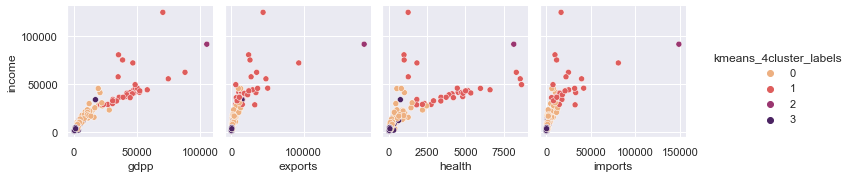
\includegraphics[scale=0.50]{income1.png}
    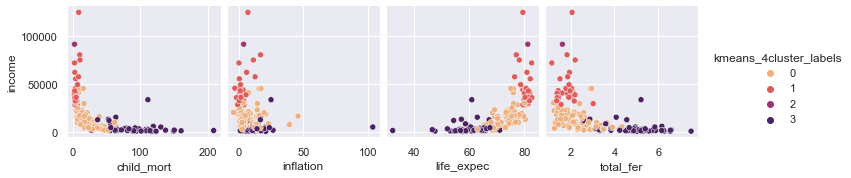
\includegraphics[scale=0.50]{income2.png}
\end{center}
We think that income is one of the most important factors affecting the development level of countries. The reason we think about this is that we can see that cluster boundaries are sharper when we visualize using income. In heatmap, the ratio of income to other columns was also high. Here, for example, the countries with the highest income and gdpp values are those in cluster 1. We can see that child mortality is high where the income value is low, and these are also the values in cluster 1. Accordingly, we can say that the countries in the cluster 1 are the most developed countries. In addition, the country in the cluster 2 is a country with high income called "Luxembourg". If we look at the bad conditions, we decided that the cluster 3 has low values in many factor such as gdpp, exports, health, imports, inflation, life expectancy and therefore it is an undeveloped country with the worst conditions. We can say that cluster 0 always has average values, therefore it includes developing countries.\\\\

\begin{wrapfigure}{r}{0.30\textwidth} 
    \vspace{\dimexpr0.05\baselineskip-\topskip}%
    \centering
    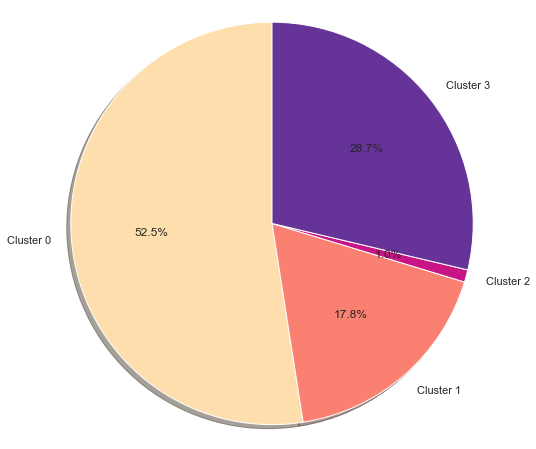
\includegraphics[width=0.35\textwidth]{percentage.png}
\end{wrapfigure}

This is a pie chart.\\
\textbf{Countries in cluster 0:} Developing countries\\ 
\textbf{Countries in cluster 1:} Developed countries\\
\textbf{Country in cluster 2:} Luxembourg\\
\textbf{Countries in cluster 3:} Undeveloped countries\\\\
As seen in the pie chart, more than half of the countries in the world are developing and we see that the number of undeveloped countries is higher than the developed ones.\\\\

\subsubsection{Showing the ratio of factors for cluster 0, 1, 3 with the help of stacked bar plot}
\begin{center}
    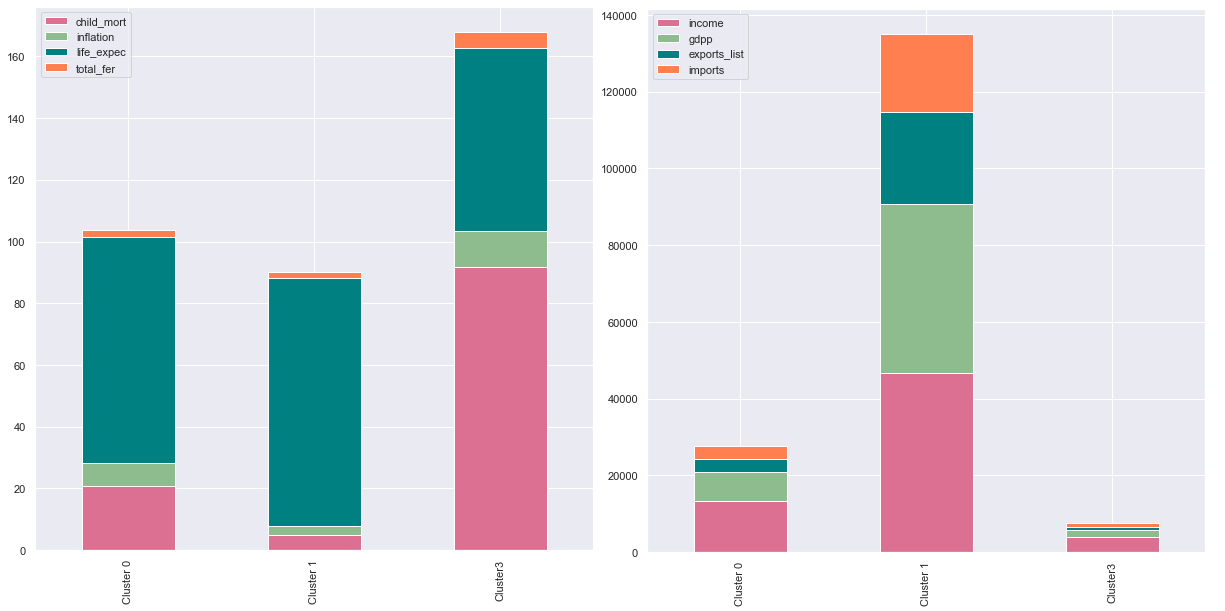
\includegraphics[scale=0.50]{stacked12.png}
\end{center}

\large
The two figures above are showing the countries in the cluster 3 with the stacked bar plot. The purpose of it to show the difference according to proportion of the factors between the countries in other clusters. For instance, we can see there are a huge amount of difference between the undeveloped countries in cluster 3 and developed countries in cluster 0. We can see the life expectancy proportion is nearly similar. Thereby we can say that life expectancy is not one of main factors to determine results. On the other hand ,factors such as child mortality or gdpp, clusters got very different proportions regarding them. To conclude, with the help of this plot, we can see the which factors are essential of determining the socioeconomic status of countries and see why the scores so low in cluster 3 comparing to other clusters clearly.

\subsubsection{Determining the top 10 undeveloped countries after k-means clustering}

\large\begin{wrapfigure}{r}{0.30\textwidth} 
    \vspace{\dimexpr0.05\baselineskip-\topskip}%
    \centering
    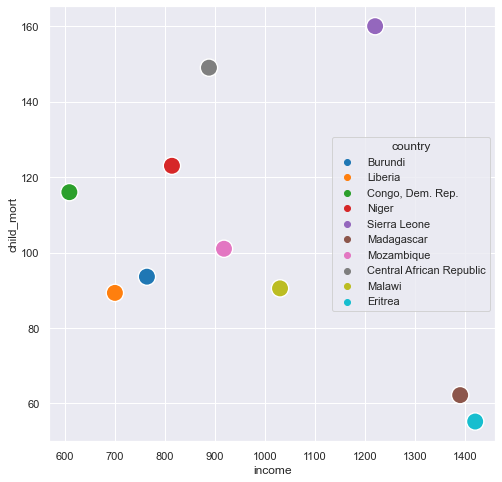
\includegraphics[width=0.35\textwidth]{10country.png}
\end{wrapfigure}

Now, we know that cluster 3 belongs to the underdeveloped countries. Here, we wanted to see the 10 worst among these underdeveloped countries. In these countries, we wanted to see the child mortality and income rate which we have always based on. While ranking these 10 countries, we ranked them according to some column values being high and others low, and then, we found these countries. Furthermore, when we look at the income scale for all countries, it has dropped dramatically from  120,000s to the 1400s. When we visualized this situation above, cluster 3 was on the top left, so there was no major change in child mortality values.

\subsection{Hierarchical Clustering}
Hierarchical clustering, also known as hierarchical cluster analysis, is an algorithm that groups similar objects into groups called clusters. The endpoint is a set of clusters, where each cluster is distinct from each other cluster, and the objects within each cluster are broadly similar to each other.\\\\
In the first figure, if we cut the dendrogram at score 8, 9 or 10, we have 4 clusters. Only at higher score of 20, 2 sets of clusters available. In the second figure, we made a drawing with 4 clusters. However, in this cluster number, it did a different clustering compared to the previous ones. As seen, developing countries merged with undeveloped ones.
Then, we thought that when we count the lines by drawing from score 6, there should be 6 clusters. This indicates 6 clusters is a good choice as there will be good dissimilarity between clusters and good similarity within clusters. When we draw it, this time, it clustered correctly. Let's move on to the results now.\\

\begin{center}
    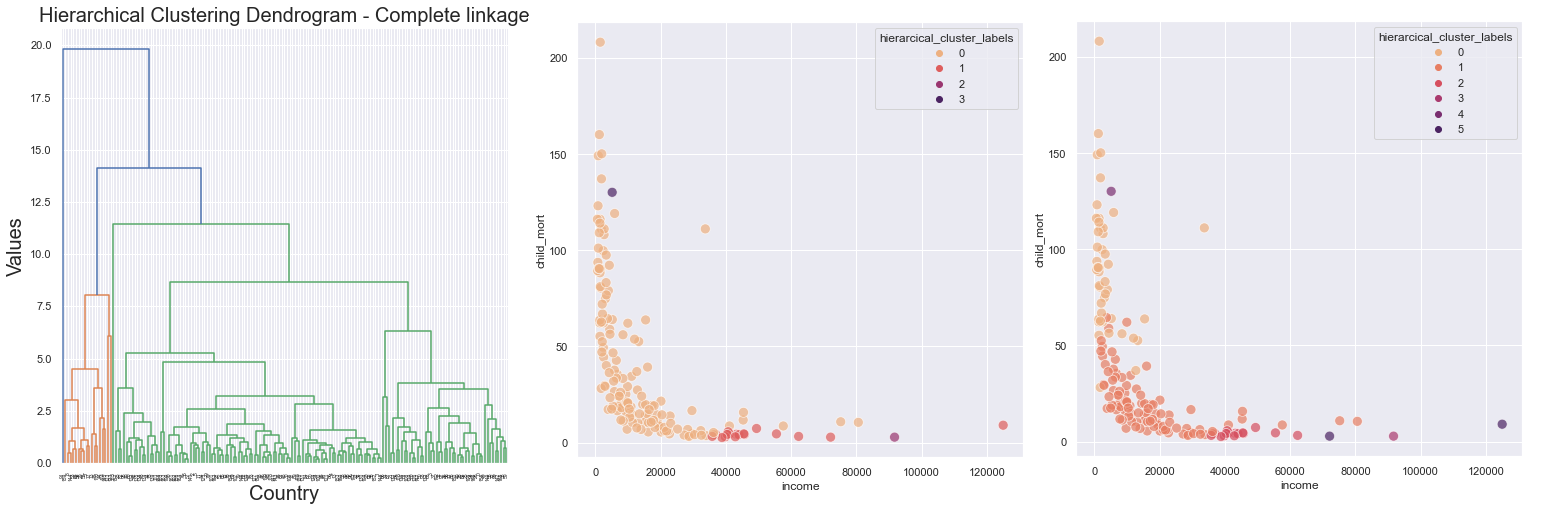
\includegraphics[scale=0.50]{hierfinal.png}
\end{center}

\section{The growth of countries' socioeconomic scores by years}

SES (Socioeconomic scores) are the average of each country's income and education ranking and are reported as percentile rankings ranging from 1-99. In this section, we will examine the growth of countries' socioeconomic scores. This score allows us to see how the countries have developed and progressed by years. We have worked on an additional dataset for this. First, we made the steps to see growth. Then, we decided to do k-means according to their voice growth. Our expectation is to see the change over the years in these countries that we have identified as undeveloped. After clustering, we wondered if they would be in the same cluster again. Before clustering, we checked the silhouette score again for 2,3,4,5,6,7,8 clusters and decided that the most correct value was 6 as shown below.

\begin{center}
    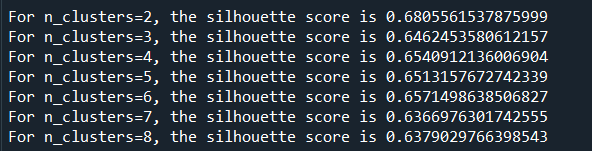
\includegraphics[scale=0.90]{ses_silüet.PNG}
\end{center}

After making K-means with 6 clusters, we printed the growth values for undeveloped countries and which cluster they are in. In addition, we printed the countries with the most progress to see the difference.

\begin{center}
    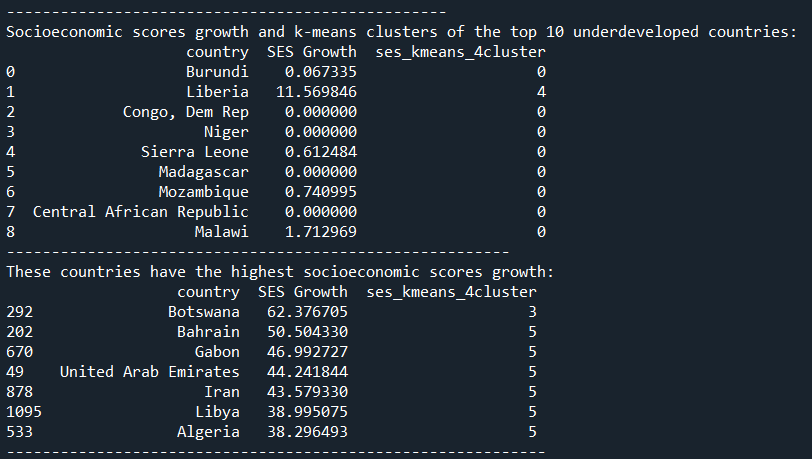
\includegraphics[scale=0.70]{ses.PNG}
\end{center}

As you can see above, the countries that are in the same cluster when we applied k-means to the first dataset, were also end up in the same cluster when we applied k-means with the dataset by years.Except for Liberia but it can be ignored. We can say that these countries could not be able to make progress through years and have difficulty in making progress. When we looked into these countries' low growth level by years, we can see why they have so low scores for the socioeconomic factors. Also the countries in the developed countries' clusters were end up in the same cluster with each other too. Another thing is the difference between developed and undeveloped countries are astonishingly high regarding to their SES growth levels. We can see that these countries make little progress through more than 100 years, so these outcomes strengthen our statement that these countries are undeveloped countries.
\section{Results}

\begin{center}
    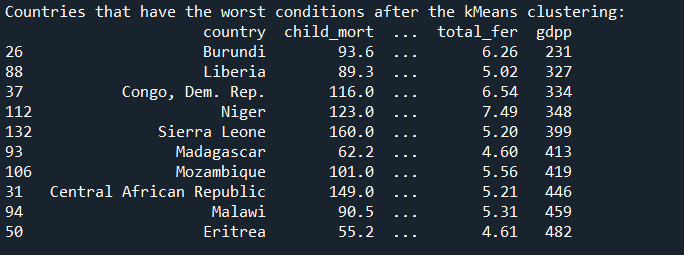
\includegraphics[width=0.55\textwidth]{10c.png}
    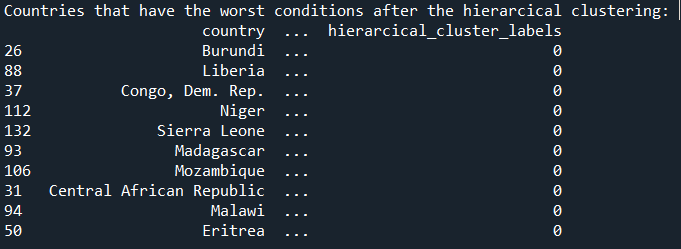
\includegraphics[width=0.55\textwidth]{hier3.png}  
\end{center}

As shown on the side, we found the same 10 underdeveloped countries as a result of both clustering. This shows that the results we found are valid. While determining the development of these countries, we looked at the following reasons.
\begin{itemize}
    \item High child mortality
    \item Low Income
    \item Low GDP
    \item Low health spent
    \item High Inflation
    \item Lower life expectancy\\\\
\end{itemize}

\section{Conclusion}

\begin{center}
    
\includegraphics[scale=1.0]{result.png}\\
\end{center}
\normalsize

\large
To conclude what we have done in the project, we have a lots points to make. Firstly, the purpose of the project is to find the countries that has the worst conditions regarding to socioeconomic factors and in the end we can clearly see that the method we choose to achieve that, clustering, is very appropriate approach. All the countries are in a cluster and these clusters are representing these countries conditions. As you can see the code above, you can enter a country and see which cluster it belongs. Moreover, one of the many importing things is how to group these countries and how many clusters would be out there. We applied the k-means algorithm on 2 datasets and we noticed that the 10 most underdeveloped countries we found in the results were both in the same cluster.\\

We get the importance of not to choose values random and by chance but make sure that we get the right value by using the tools such as elbow curve, silhouette score and Hopkins score. This lead the another crucial lesson we get from this project which is how the algorithm choices of the programmer effect the outcome. For instance, number of clusters might have huge consequences. If the cluster number was too low, some underdeveloped countries may end up in developing countries and will not be considered qualified for aid from international organisations. Also separating the ones with unusual values because, they will chance the proportion of the data and results. With the projects that holds such crucial roles like, it is important to try different methods in addition and comparing them. We also applied hierarchical clustering and got the same countries as k-mean clustering.


In such a real-life data, visualization is crucial. Figures must be visible and understandable so that we can analyze the figures easily. Thanks to this project, we learned which visualization types we can use in which situations. We have seen that the types used for displaying figures such as pie chart, stacked bar plot will be more useful when we use them to show what situation. In addition, we have learned that how we can write figures' code from both "seaborn" and "matplotlib" libraries.\\


There are factors that we know proportionally in real life, for example, it is a situation that everyone agrees that child mortality should increase as income decreases. We analyzed which factors really correlate negatively and positively with which factors, thanks to the heatmap.
One of the outcomes we get is that most of the countries around the world are developing countries. The number of undeveloped countries is quite high. When we look at the results, these undeveloped countries are mostly African countries. As a result, we think that African countries should be focused on among the countries that need to be helped.\\


Furthermore, as a result of the stacked bar plot figure in 4.1.6, we see that the development of the health and economy sectors is higher in clusters of developed and developing countries. Countries in Cluster 3 can develop their countries if they invest in these sectors. \\


\emph{For us, this project was a good example of how to use the programming and data mining for the greater good and in the future, we hope there will be lots of more examples with extended features and data.}
\nocite{*}
\bibliographystyle{plain}
\bibliography{references}
\end{document}

